\documentclass[preprint,11pt]{elsarticle}
\usepackage{amsmath,amssymb,amsthm,graphicx,booktabs,array,tabularx,longtable}
\usepackage{algorithm,algpseudocode,tikz}
\usetikzlibrary{arrows.meta,positioning,calc,fit,backgrounds}
\usepackage[T1]{fontenc}
\usepackage{lmodern}
\usepackage[margin=1in]{geometry}
\usepackage{microtype}
\usepackage[hidelinks]{hyperref}
\theoremstyle{definition}\newtheorem{definition}{Definition}[section]
\theoremstyle{plain}
\newtheorem{theorem}{Theorem}\newtheorem{lemma}{Lemma}
\newtheorem{corollary}{Corollary}\newtheorem{proposition}{Proposition}
\theoremstyle{remark}\newtheorem{remark}{Remark}[section]
\newcommand{\negl}{\mathsf{negl}}\newcommand{\Adv}{\mathsf{Adv}}
\newcommand{\ppt}{\mathsf{PPT}}\newcommand{\Absorb}{\mathrm{Absorb}}
\newcommand{\sid}{\mathsf{sid}}\newcommand{\pid}{\mathsf{pid}}
\emergencystretch=1.5em

\hypersetup{pdftitle={Radix-Packed Multi-Record Retrieval over an XPIR-Style RLWE Interface},pdfauthor={Hao-Yi Hsu, Po-Chun Su, Raylin Tso, Jen-Chieh Hsu}}
\begin{document}
\begin{frontmatter}
\title{Radix-Packed Multi-Record Retrieval over an XPIR-Style RLWE Interface}
\author[nccu]{Hao-Yi Hsu}\ead{d11201@cs.nccu.edu.tw}
\author[nccu]{Po-Chun Su}\ead{111753133@g.nccu.edu.tw}
\author[nccu]{Raylin Tso\corref{corresponding}}\ead{raylin@cs.nccu.edu.tw}
\author[nccu]{Jen-Chieh Hsu}\ead{105753501@nccu.edu.tw}
\cortext[corresponding]{Corresponding author.}
\affiliation[nccu]{organization={Department of Computer Science, National Chengchi University},country={Taiwan}}
\begin{abstract}

Retrieving several records privately can duplicate query and evaluation
work, even when single-record requests run concurrently. We study radix
packing within an XPIR-style RLWE interface: one encrypted selector
vector retrieves an ordered tuple, with bounded record segments combined
in each reply coefficient. The construction specifies record encoding,
exact plaintext capacity and digit recovery. We prove correctness under
an integer no-wrap condition and derive a parametric full-task failure
bound for a specified rounded Gaussian law. Single-challenge index privacy
reduces to uniform-secret decisional PLWE with one additional ring sample
and an explicit unit-probability loss. These claims do not certify the
native sampler or concrete security. On a WSL2 host, a controlled
two-record comparison against concurrent same-profile repeated XPIR covers
48 workload/profile points in cold and online views. Median paired
repeated-to-packed task latency ratios range from 1.059 to 1.190; all 96
pointwise bootstrap intervals exceed one. Separate multiplicity,
implementation/resource sensitivity and capacity experiments extend the
finite evidence, including one two-block workload, without pooling their
samples. Packing reduces native ciphertext buffers relative to repeated
execution, while the flat query remains larger than the raw database at
the reported lengths. The results characterize a restricted instantiation
of prior weighted retrieval; the native/formal reliability bridge and
transport performance remain open.

\end{abstract}
\begin{keyword}
Private information retrieval \sep RLWE \sep radix packing \sep XPIR \sep index privacy
\end{keyword}
\end{frontmatter}
\raggedbottom
\section{Introduction}
\label{sec:intro}
Private information retrieval (PIR) hides a client's requested indices
from the server~\cite{chor1998private,kushilevitz1997replication}.
When one task needs several records, repeating a single-record protocol
also repeats query generation, evaluation and extraction. Concurrent
execution can overlap that work, so reducing the number of queries alone
does not establish a completed-task latency benefit.

This paper studies a restricted alternative within the linear evaluation
interface of XPIR~\cite{melchor2016xpir}. The client encrypts one weighted
selector vector for an ordered tuple of distinct indices. Each record
is divided into bounded integer segments and encoded into polynomial
coefficients. Public radix weights place the selected segments in
different digit positions of each reply coefficient, allowing ordinary
digit extraction after decryption. A query is one vector of \(N\)
ciphertexts, not a compressed single ciphertext; the reply contains
one ciphertext per polynomial block.

Encrypted weighted multi-value retrieval is established prior
work~\cite{mulityquery}, and radix representation is standard. The question
here is how to specify its encoding, capacity and integer-noise conditions
for an XPIR-style RLWE interface, and what performance this instantiation
exhibits against concurrent same-profile repeated retrieval. Coefficient
capacity, backend API support and finite functional execution are distinct
constraints. In particular, a formal law cannot be inferred from a
native sampler merely because observed replies decode correctly.

The paper makes three contributions:
\begin{itemize}
\item An explicit record-to-polynomial radix construction, with ordered
recovery, exact capacity \(t\ge B^\alpha\), zero padding and a native
interface retaining XPIR's linear reply arithmetic.
\item Scoped formal analysis: conditional integer no-wrap correctness,
a parametric full-task bound for a specified rounded Gaussian law, and
single-challenge index privacy from uniform-secret decisional PLWE with
\(N+1\) samples and explicit unit-probability loss.
\item Separate controlled evaluations of two-record task latency,
multiplicity, implementation/resource sensitivity and capacity, together
with reproducible native-buffer accounting and functional checks.
\end{itemize}

The primary two-record comparison covers 48 workload/profile points in
both cold and online views. Its median paired repeated-to-packed latency
ratios range from 1.059 to 1.190, with all 96 pointwise intervals above
one. Further experiments extend multiplicity and block coverage under
their own contracts; they are not pooled with the primary evidence.
These findings concern a fixed profile and host. They establish neither
a global XPIR optimum nor superiority over other PIR systems, and the
native/formal sampler and reliability bridge remains unresolved.

\section{Related Work}
\label{sec:related-work}

\subsection{XPIR and RLWE-based PIR}
XPIR~\cite{melchor2016xpir} is the closest backend reference. Its
homomorphic query and database evaluation support efficient polynomial
arithmetic, and its broader design includes aggregation and recursion.
Our scope retains the one-dimensional linear path, with a direct SKE
selector vector and explicit coefficient layout. This restricted path
does not exhaust XPIR's optimization space. The empirical conclusions below
concern concurrent same-profile repeated XPIR. No measured superiority
across all XPIR configurations is claimed. The pinned implementation~\cite{xpir_github} establishes
artifact provenance, not a substitute citation for the XPIR paper or
evidence that its native sampler realizes our formal distribution.

\subsection{Multi-value and Weighted Retrieval}
Hsu et al.~\cite[Secs.~III--V]{mulityquery} are the closest conceptual
prior work. Their group-homomorphic construction already supports an
encrypted weight at each selected position, encryptions of zero elsewhere,
a homomorphic weighted sum, and client-side recovery of two or more
values. They also discuss retrieval-count limits imposed by the plaintext
modulus and a privacy argument from the underlying encryption security.
Neither the multi-value goal nor that generic weighted architecture is
new here.

The positional weights \(K=(1,B,\ldots,B^{\alpha-1})\) are public and
target-independent. This instantiation replaces growing-weight
remainder recovery with ordinary radix digit extraction. Radix itself is
standard. The research increment is the precise connection between this
choice, record-to-polynomial encoding, exact capacity and the integer
no-wrap condition of the XPIR-style RLWE interface. The aggregate error
depends on all encoded database polynomials, whereas direct encryption of
a weight does not scale its encryption error by that weight. The formal
privacy reduction and native mapping concern this instantiation; generic
homomorphic privacy arguments and modulus limitations already occur in
the prior work. The conditional theorem alone establishes no concrete
security-admissible region. The separately tested native API frontier in
Section~\ref{sec:native-validation} concerns implementation feasibility and
finite functional execution, not a native noise or security certificate.

\subsection{Batch, SIMD, and Preprocessed PIR}
Angel et al.~\cite{angel2018pir} introduce SealPIR's compressed queries
and, separately, probabilistic batch codes (PBCs) for amortizing a batch.
The latter distribute encoded database items across buckets and use a
retrieval schedule, including cuckoo placement. SealPIR and the PBC
transformation are separate contributions in that same paper.
Vectorized BatchPIR~\cite{vectorized2023} uses vectorized RLWE homomorphic
encryption, bucketed batch retrieval, SIMD operations and ciphertext merging.
PIRANA~\cite{pirana2024} combines constant-weight index encoding with
homomorphic slot operations and a batch-code route; rotations and response
organization depend on the payload and configuration. Their setup,
evaluation keys and placement failure models matter to a comparison.

SimplePIR and DoublePIR are two protocols in the same
paper~\cite{henzinger2023one}. They use LWE-based linear processing with
database-dependent hints downloaded by the client; DoublePIR trades
additional processing for a smaller hint. Online work cannot be compared
to an entire fresh task while omitting this state and its lifecycle.
These protocols provide preprocessing context rather than the direct
weighted-packing precedent.

Respire~\cite[Secs.~2--4]{respire2024} directly studies small records and
batch queries. It uses subrings, ring switching, query compression and
response packing, and composes with PBCs for batch retrieval. Its model
includes reusable client query-key material and server database
preprocessing. SPIRIT~\cite[Secs.~2--5]{spirit2026} combines PBC scheduling
with LWE-to-RLWE conversion, shared key-expansion state and response
compression. Its hintless online interface does not mean absence of
server preprocessing or state. Thus neither short-record support,
small-batch access, lack of an offline client hint nor response packing
alone distinguishes the present work.

\begin{table}[t]
\centering
\caption{Mechanism summary, without a performance ranking. State and
assumptions differ across rows. The artifact provides an expanded mechanism comparison.}
\label{tab:mechanisms}
\small
\setlength{\tabcolsep}{3pt}
\begin{tabular}{@{}>{\raggedright\arraybackslash}p{2.0cm}>{\raggedright\arraybackslash}p{4.1cm}>{\raggedright\arraybackslash}p{4.7cm}@{}}
\toprule
Scheme & Retrieval mechanism & Relation to this study \\
\midrule
XPIR & Encrypted selection; linear evaluation; optional aggregation/recursion & Backend and empirical comparator; current path is flat. \\
Hsu et al. & Encrypted weights, weighted sum and integer recovery & Closest generic multi-value precedent; modulus/count limits already studied. \\
SealPIR / PBC & Compressed queries; separate bucketed batch transformation & Compression and placement are distinct mechanisms. \\
Vectorized BatchPIR & Bucket placement, SIMD processing and ciphertext merging & Batch alternative; not a local timing baseline. \\
PIRANA & Constant-weight selection, slots/rotations and batch codes & Alternative batch organization and payload tradeoffs. \\
SimplePIR / DoublePIR & LWE linear processing with client-downloaded hints & Preprocessing and amortization context. \\
Respire & Subring/ring-switching compression and response packing; batch codes & Direct short-record and small-batch precedent. \\
SPIRIT & PBCs, stateful ciphertext conversion and packed responses & Direct hintless-batch and response-packing precedent. \\
This construction & Several scalar digits per coefficient; unchanged linear ReplyGen & Restricted instantiation; capacity/noise/backend feasibility remains central. \\
\bottomrule
\end{tabular}
\end{table}


Radix packing here separates records by integer digit positions within
each coefficient, without bucket placement or SIMD rotations to recover
the targets. These architecture properties do not imply lower latency,
memory or failure probability. The contribution is the explicit
encoding/capacity/noise connection and its scoped evaluation within
XPIR, rather than query compression, offline hints or large-batch
optimization. External schemes provide mechanism and state context;
their published timings are not mixed with the local measurements.

\section{Preliminaries and Problem Model}
\label{sec:preliminaries}
\subsection{Notation and Public Parameters}
\label{sec:notation-params}
For a positive integer \(d\), write \([d]=\{1,\ldots,d\}\).
The security parameter is \(\kappa\); PPT means probabilistic polynomial time.
For an integer \(z\) and modulus \(d\ge2\), \([z]_d\) is its canonical
representative in \(\{0,\ldots,d-1\}\). This notation extends coefficient-wise.
For a monic polynomial \(f\in\mathbb Z[X]\) of degree \(n\), write
\[
 R=\mathbb Z[X]/(f),\qquad R_q=R/qR,\qquad R_t=R/tR.
\]
The construction uses \(f=X^n+1\), with \(n\) a power of two,
\(t=2^w\), \(q>t\), and \(\gcd(t,q)=1\).
The privacy reduction does not require \(q\) to be prime.
All parameter descriptions have polynomial bit length in \(\kappa\);
ring degrees and sample counts in the reductions are polynomially bounded.
Every ring element has a unique representative of degree less than \(n\).
For \(P\in R_t\), \(\widehat P\in R\) denotes the lift whose coefficients
lie in \([0,t)\). This lift, followed by reduction modulo \(q\), is an
encoding into \(R_q\), not a ring homomorphism from \(R_t\).
For \(z\in R_q\), \(\operatorname{center}_q(z)\in R\) is obtained by choosing
each coefficient in \([-q/2,q/2)\). The infinity norm in \(R\) is the maximum
absolute value of its integer coefficients.

\begin{table}[t]
\centering
\caption{Public parameters and encoding units.}
\label{tab:notation}
\small
\begin{tabular}{@{}lp{8.9cm}@{}}
\toprule
Symbol & Meaning \\
\midrule
\(N,n\) & Number of database records; coefficients per polynomial (\(n\) a power of two). \\
\(\ell,\rho_0\) & Original record length and segment width, in bits; both at least one. \\
\(B,w,t\) & Segment bound \(B=2^{\rho_0}\); selected backend coefficient width \(w\); \(t=2^w\). \\
\(J,L\) & Segments per record \(J=\lceil\ell/\rho_0\rceil\); polynomial blocks per record \(L=\lceil J/n\rceil\). \\
\(\alpha,K\) & Number of distinct targets, \(1\le\alpha\le N\); derived radix weights \(K=(1,B,\ldots,B^{\alpha-1})\). \\
\(\ell_{\rm enc}\) & Full-block encoded bit length \(Lnw\); distinct from \(\ell\) and \(Jw\). \\
\(\chi_r,r\) & Coefficient-wise rounded Gaussian family and its public continuous standard deviation \(r>0\); \(\chi_s=\chi_e=\chi_r\). \\
\(p_{\rm unit}\) & Probability that a uniform element of \(R_q\) is invertible. \\
\bottomrule
\end{tabular}
\end{table}

The public parameters \(pp\) specify \(\kappa,N,f,n,q,t,w,\ell,\rho_0,\alpha,K\),
the public width \(r>0\), the family \(\chi=\chi_r\) defined below, and the
encoding layout; \(B,K,J,L\) are derived, with \(k_\nu=B^{\nu-1}\), \(\nu\in[\alpha]\). We retain
\(\chi_s=\chi_e=\chi_r\) as aliases in the construction and its separate
correctness statement. All public parameters are fixed independently
of the secret target tuple. In particular, \(pp\)
is not a public encryption key. The exact radix capacity condition is
\(t\ge B^\alpha\), equivalently \(w\ge\alpha\rho_0\), as in
Lemma~\ref{lemma:packing-condition}. The weights are canonical elements of
\(\mathbb Z_t\), not necessarily units; no weight coprimality or inverse
is required. The condition \(\gcd(t,q)=1\) remains necessary for the
security reduction. 

\subsection{Retrieval Task and Interfaces}
\label{sec:mq-model}
A legal database is an ordered list \(M=(m_1,\ldots,m_N)\in
(\{0,1\}^{\ell})^N\). A legal request is an ordered tuple
\(I=(i_1,\ldots,i_\alpha)\in[N]^\alpha\) of pairwise-distinct indices;
record contents at distinct indices may be equal. Write
\(M[I]=(m_{i_1},\ldots,m_{i_\alpha})\).
The deterministic record map \(\mathsf{Encode}:\{0,1\}^{\ell}\to R_t^L\)
is specified in Section~\ref{sec:encoding}. We use
\(\mathsf{DBEncode}(M)=(\mathsf{Encode}(m_i))_{i\in[N]}\)
only as its row-wise abbreviation, not as an additional protocol.

\begin{table}[t]
\centering\small
\caption{Protocol interfaces and ownership. Public parameters determine all
dimensions. Query generation is randomized; reply generation and extraction
are deterministic for their inputs.}
\label{tab:interfaces}
\begin{tabularx}{\linewidth}{@{}llX@{}}
\toprule Algorithm & Party & Input and output \\
\midrule
\(\mathsf{KeyGen}\) & Client & \(pp\mapsto sk=s\); one fresh secret per query. \\
\(\mathsf{QueryGen}\) & Client & \((pp,sk,I)\mapsto(Q,\mathsf{st})\), where
\(Q\in(R_q^2)^N\) and private \(\mathsf{st}=I\). \\
\(\mathsf{ReplyGen}\) & Server & \((pp,P,Q)\mapsto\mathsf{Resp}\in(R_q^2)^L\),
where \(P=\mathsf{DBEncode}(M)\in R_t^{N\times L}\). \\
\(\mathsf{ReplyExt}\) & Client & \((pp,sk,\mathsf{Resp},\mathsf{st})\mapsto
\widehat M\in(\{0,1\}^{\ell})^\alpha\), in the requested order. \\
\bottomrule
\end{tabularx}
\end{table}
Only \(Q\) leaves the client; \(sk\) and \(\mathsf{st}\) remain private.
A single query is a vector of \(N\) ciphertexts, and the response contains
\(L\) ciphertexts. Public parameters, including the encoding and weights,
are fixed independently of the target tuple.

\subsection{Correctness Goal}
For every admissible \(pp\), legal \(M\), and legal \(I\), consider the
honest execution
\[
 sk\leftarrow\mathsf{KeyGen}(pp),\quad
 (Q,\mathsf{st})\leftarrow\mathsf{QueryGen}(pp,sk,I),
\]
\[
 \mathsf{Resp}=\mathsf{ReplyGen}(pp,\mathsf{DBEncode}(M),Q),\quad
 \widehat M=\mathsf{ReplyExt}(pp,sk,\mathsf{Resp},\mathsf{st}).
\]
Define \(\mathrm{Corr}=[\widehat M=M[I]]\). A correctness target
\(\Pr[\neg\mathrm{Corr}]\le\delta_{\rm corr}(pp)\) quantifies over all
such databases and requests, with probability over key generation and
all encryption randomness. This target is a specification, not an
unconditional negligible-failure claim. Section~\ref{sec:corr} proves
ordered recovery under an integer no-wrap condition and derives a bound
for the specified error law.

\subsection{Single-challenge Index Privacy}
\label{sec:mq-privacy}
\begin{definition}[Index privacy for packed multi-record retrieval]
\label{def:mq-cpir-privacy}
Fix admissible public parameters \(pp\) independently of the targets. The database and target tuples must be legal as defined above; both
challenge tuples use the same public layout and weight tuple. For a two-stage PPT adversary \(\mathcal A=(\mathcal A_1,\mathcal A_2)\),
the experiment is:
\begin{enumerate}
\item The challenger samples \(sk\leftarrow\mathsf{KeyGen}(pp)\).
\item \(\mathcal A_1(pp)\) outputs \((M,I_0,I_1,\sigma)\), where \(\sigma\)
is its polynomial-length private state. Both tuples and the database must be
legal. The tuples may coincide, covering degenerate instances such as
\(N=\alpha=1\). On illegal input, the experiment terminates with an independent
fair success bit.
\item The challenger samples \(b\leftarrow\{0,1\}\), computes
\[
 (Q,\mathsf{st})\leftarrow\mathsf{QueryGen}(pp,sk,I_b),\qquad
 P=\mathsf{DBEncode}(M),
\]
\[
 \mathsf{Resp}=\mathsf{ReplyGen}(pp,P,Q),
\]
and gives \((Q,\mathsf{Resp})\) to the adversary.
\item \(b'\leftarrow\mathcal A_2(pp,M,I_0,I_1,\sigma,Q,\mathsf{Resp})\).
The experiment succeeds iff \(b'=b\).
\end{enumerate}
Neither \(sk\) nor the client state \(\mathsf{st}\) is disclosed. Define
\[
 \Adv^{\rm priv}_{\Pi,\mathcal A}(\kappa)
   =\left|\Pr[\text{experiment succeeds}]-\tfrac12\right|.
\]
Single-challenge index privacy means this advantage is negligible for every
PPT adversary. The probability includes key generation, all encryptions,
the challenge bit, and adversary randomness.
\end{definition}
The public parameters, database, and adversary state are part of the server's
view. Its deterministic intermediate computations are functions of these
values and the query. No decryption outcome or client extraction state is
included in this game.

\subsection{Specified Error Law}
We adopt the coefficient-wise Gaussian family explicitly defined by
Brakerski and Vaikuntanathan~\cite[Sec.~1.3]{homomorphic}:
\[
 Y_j\leftarrow\mathcal N(0,r^2),\qquad
 Z_j=\operatorname{round}(Y_j),\qquad
 \chi_r=\mathcal L\!\left(\sum_{j=0}^{n-1}Z_jX^j\right),
\]
where the \(Y_j\) are independent and rounding is to the nearest integer.
Equivalently, one coefficient has probability mass
\[
 p_r(z)=\int_{z-1/2}^{z+1/2}
       \frac{\exp(-y^2/(2r^2))}{\sqrt{2\pi}\,r}\,dy,\qquad z\in\mathbb Z.
\]
Half-integer ties have probability zero under the ideal continuous law.
Both the secret and every fresh encryption error use this same
product distribution, independently across coefficients and draws.
Here \(r\) is the standard deviation before rounding; its numerical value
remains to be selected jointly with the other parameters.


This rounded law differs from the integer Gaussian with mass proportional
to \(\exp(-\pi z^2/\eta^2)\) and is not identified here with a
canonical-embedding Gaussian. Efficient machine realization and its
approximation to this ideal law require separate justification.

\subsection{Linear Encryption Interface}
\label{sec:prelim}
We use the symmetric-key algebraic interface of the Ring-LWE construction
of Brakerski and Vaikuntanathan~\cite{homomorphic}, in the linear evaluation
setting of XPIR~\cite{melchor2016xpir}. All ciphertext arithmetic below is in
\(R_q\); all message lifts use canonical coefficients.
\begin{align*}
 \mathsf{KeyGen}(pp)&:\ s\leftarrow\chi,\quad sk=s,\\
 \mathsf{Enc}_s(v)&:\ a\leftarrow R_q\text{ uniformly},\quad e\leftarrow\chi,
   \quad C=(as+te+\widehat v,-a),\\
 \mathsf{Dec}_s(C)&:=
   [\operatorname{center}_q(c_0+c_1s)]_t,\\
 \mathsf{Add}(C,C')&:=(c_0+c'_0,c_1+c'_1),\\
 \Absorb(P,C)&:=(\widehat P c_0,\widehat P c_1).
\end{align*}
Each encryption samples fresh independent \(a,e\), including encryptions of
zero. The client alone possesses \(sk\), encrypts queries, and decrypts
replies. The server needs only \(pp\), the encoded database, and ciphertexts
to perform \(\mathsf{Add}\) and \(\Absorb\). No ciphertext--ciphertext
multiplication or public key is required.

XPIR's mathematical representation \((a,b)\), with \(b=as+te+v\), corresponds
to our \(C=(b,-a)\), so \(c_0+c_1s=b-as\). This correspondence makes no claim
of identical binary serialization. The final mod-\(t\) step returns canonical
coefficients, whereas the preceding mod-\(q\) step uses centered coefficients.
Correctness requires control of the integer value before reduction modulo
\(q\), as formalized in Theorem~\ref{thm:correctness}.

\subsection{Uniform-secret Decisional PLWE}
\label{sec:rlwe-plwe}
\begin{definition}[Uniform-secret decisional PLWE]
\label{def:uplwe}
Fix a publicly specified parameter family \((f,q,\chi)\), where \(\chi\)
is efficiently sampleable over \(R\). For a polynomially bounded
\(\tau=\tau(\kappa)\), consider
\[
 \mathcal U_{\rm real}^{(\tau)}
   =((a_i,a_i s+e_i))_{i=1}^{\tau},\qquad
 \mathcal U_{\rm unif}^{(\tau)}
   =((a_i,u_i))_{i=1}^{\tau}
\]
in \((R_q^2)^\tau\). One secret \(s\leftarrow U(R_q)\) is shared by all
samples. All \(a_i,u_i\leftarrow U(R_q)\) and \(e_i\leftarrow\chi\)
are mutually independent and independent of \(s\); errors are reduced
modulo \(q\) when used in \(R_q\). For a PPT distinguisher \(\mathcal B\), define
\[
 \Adv^{\rm uPLWE}_{\mathcal B}(\kappa;\tau)=
 \left|\Pr[\mathcal B(pp,\mathcal U_{\rm real}^{(\tau)})=1]
       -\Pr[\mathcal B(pp,\mathcal U_{\rm unif}^{(\tau)})=1]\right|.
\]
The \(\tau\)-sample assumption for this family is that this advantage is
negligible in \(\kappa\) for every PPT \(\mathcal B\).
\end{definition}
This is a distribution-specific decisional assumption, following the
uniform-secret PLWE formulation discussed in~\cite[Sec.~2]{homomorphic}.
Hardness is assumed only for the corresponding instance, not for every
efficiently sampleable \(\chi\). We make no worst-case ideal-lattice
reduction claim and certify no concrete security level.

\section{Radix-Packed Retrieval}
\label{sec:proposal}
The construction represents segments from different records as digits
inside a coefficient. It uses direct encryptions of public radix weights
and retains the linear reply interface of Section~\ref{sec:prelim}.
The encoding, selector, and extraction must share the same public layout.
\subsection{Record Encoding and Decoding}
\label{sec:encoding}
Fix an ordered record \(m_i=(b_{i,0},\ldots,b_{i,\ell-1})\in\{0,1\}^{\ell}\).
Set \(b_{i,v}=0\) for \(v\ge\ell\). For \(h\in[J]\), define
\begin{equation}
\label{eq:segments}
 x_{i,h}=\sum_{v=0}^{\rho_0-1}2^v b_{i,(h-1)\rho_0+v},\qquad
 0\le x_{i,h}<B=2^{\rho_0}.
\end{equation}
Set \(x_{i,h}=0\) for \(h>J\). Thus an incomplete final segment is padded
with zero high bits. Define \(\mathsf{Encode}(m_i)=(P_{i,1},\ldots,P_{i,L})\),
where
\begin{equation}
\label{eq:encode}
 P_{i,j}(X)=\sum_{u=0}^{n-1}x_{i,(j-1)n+u+1}X^u\in R_t,
 \qquad j\in[L].
\end{equation}
The indices are \(i\in[N]\), \(j\in[L]\), \(h\in[J]\), and
\(u\in\{0,\ldots,n-1\}\); their relation is \(h=(j-1)n+u+1\).
Each coefficient holds one scalar segment, and each polynomial holds up to
\(n\) segments. The final polynomial is padded with zero coefficients.

\(\mathsf{Decode}\) reads canonical coefficients in increasing \(j\), then
increasing \(u\), keeps the first \(J\) segments, and expands each into
\(\rho_0\) bits in increasing bit position. It concatenates these bits and
retains the first \(\ell\). For the image of \(\mathsf{Encode}\), uniqueness
of the binary expansion in \([0,B)\) recovers every bit in
\eqref{eq:segments}; the discarded bits and coefficients are precisely the
padding. Consequently
\[
 \mathsf{Decode}(\mathsf{Encode}(m_i))=m_i.
\]

\subsection{Packed Reply Structure}
\label{sec:overview}
For target ordinal \(\nu\in[\alpha]\), associate \(i_\nu\) with
\(k_\nu=B^{\nu-1}\). The intended plaintext of reply block \(j\) is
\begin{equation}\label{eq:packed-plaintext}
 PM_j=\sum_{\nu=1}^{\alpha}k_\nu P_{i_\nu,j}\in R_t.
\end{equation}
The client decrypts each block, extracts the canonical radix digits,
and decodes the resulting record polynomials (Fig.~\ref{fig:system-overview}).
\begin{figure}[t]
\centering
\resizebox{\linewidth}{!}{%
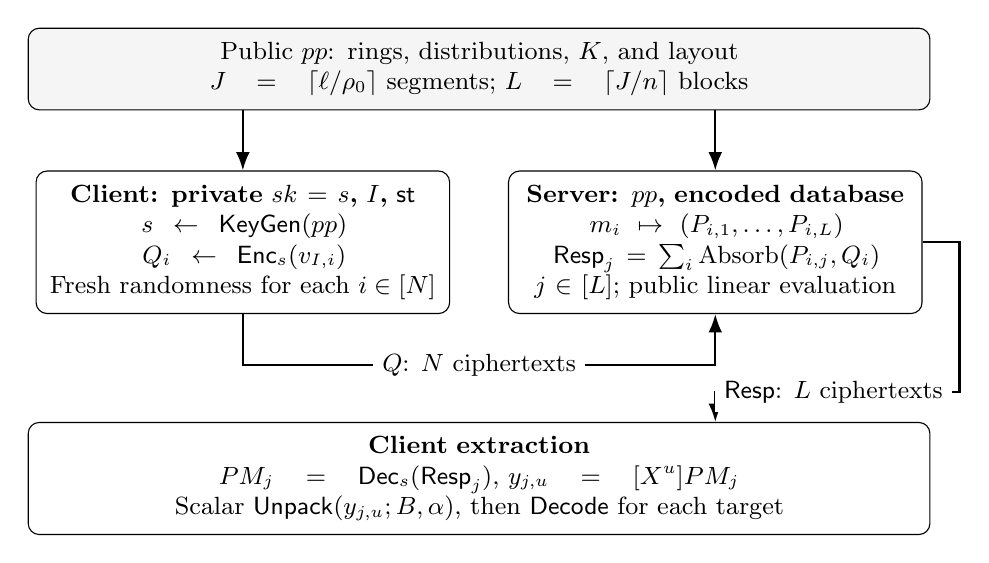
\begin{tikzpicture}[
 font=\small,>=Latex,
 box/.style={draw,rounded corners,align=center,text width=4.9cm,inner sep=5pt},
 flow/.style={-{Latex},thick}]
\node[box,text width=11.1cm,fill=black!4] (pp) at (0,0)
 {Public \(pp\): rings, distributions, \(K\), and layout\\
 \(J=\lceil\ell/\rho_0\rceil\) segments; \(L=\lceil J/n\rceil\) blocks};
\node[box] (client) at (-3,-2.2)
 {\textbf{Client: private \(sk=s\), \(I\), \(\mathsf{st}\)}\\
 \(s\leftarrow\mathsf{KeyGen}(pp)\)\\
 \(Q_i\leftarrow\mathsf{Enc}_s(v_{I,i})\)\\
 Fresh randomness for each \(i\in[N]\)};
\node[box] (server) at (3,-2.2)
 {\textbf{Server: \(pp\), encoded database}\\
 \(m_i\mapsto(P_{i,1},\ldots,P_{i,L})\)\\
 \(\mathsf{Resp}_j=\sum_i\Absorb(P_{i,j},Q_i)\)\\
 \(j\in[L]\); public linear evaluation};
\node[box,text width=11.1cm] (ext) at (0,-5.2)
 {\textbf{Client extraction}\\
 \(PM_j=\mathsf{Dec}_s(\mathsf{Resp}_j)\), \(y_{j,u}=[X^u]PM_j\)\\
 Scalar \(\mathsf{Unpack}(y_{j,u};B,\alpha)\), then \(\mathsf{Decode}\) for each target};
\draw[flow] (pp.south -| client.north) -- (client.north);
\draw[flow] (pp.south -| server.north) -- (server.north);
\draw[flow] (client.south) -- ++(0,-0.65) -| (server.south)
 node[pos=0.25,fill=white] {\(Q\): \(N\) ciphertexts};
\draw[flow] (server.east) -- (6.1,-2.2) -- (6.1,-4.1)
 -- (3,-4.1) -- (ext.north -| server.south);
\node[fill=white] at (4.5,-4.1) {\(\mathsf{Resp}\): \(L\) ciphertexts};
\end{tikzpicture}%
}
\caption{SKE query--reply--extraction flow. Secret-key generation and client
state are local to the client. Each reply encrypts one packed polynomial
\(PM_j\), containing up to \(n\) packed scalar coefficients; decryption
and extraction are correct under Theorem~\ref{thm:correctness}.}
\label{fig:system-overview}
\end{figure}
\subsection{Scalar Packing and Unpacking}
\label{sec:param}
\begin{lemma}[Radix packing/unpacking]
\label{lemma:packing-condition}
Let \(B=2^{\rho_0}\), \(\rho_0\ge1\), \(\alpha\ge1\), and
\(x_{\nu}\in\{0,\ldots,B-1\}\). Set
\begin{equation}
\label{eq:weights}
 K=(1,B,\ldots,B^{\alpha-1}),\qquad k_{\nu}=B^{\nu-1}.
\end{equation}
Then \(y=\sum_{\nu=1}^{\alpha}B^{\nu-1}x_{\nu}\) satisfies
\(0\le y<B^\alpha\), has a unique base-\(B\) representation, and
\(\mathsf{Unpack}(y;B,\alpha)\) returns its digits by
\begin{equation}
\label{eq:unpack}
 x_{\nu}=\left\lfloor\frac{y}{B^{\nu-1}}\right\rfloor\bmod B,
 \qquad \nu\in[\alpha].
\end{equation}
All such integers embed without reduction in \(\mathbb Z_t\) exactly when
\(t\ge B^\alpha\). For \(t=2^w\), this is equivalent to
\(w\ge\alpha\rho_0\).
\end{lemma}
\begin{proof}
The geometric sum gives
\[
 0\le y\le(B-1)\sum_{\nu=1}^{\alpha}B^{\nu-1}=B^\alpha-1.
\]
For each \(\nu\), the contribution from lower positions is less than
\(B^{\nu-1}\), while each higher position is a multiple of \(B^{\nu}\).
Integer division by \(B^{\nu-1}\), followed by reduction modulo \(B\),
therefore returns exactly \(x_{\nu}\). This deterministic inverse proves
uniqueness. Conversely, every integer in \([0,B^\alpha)\) has these
\(\alpha\) digits, so the domain has exactly \(B^\alpha\) values.
Its canonical embedding into \([0,t)\) is possible exactly when
\(t\ge B^\alpha\), including equality. When \(\alpha=1\),
\(K=(1)\) and the decoder returns \(x_1=y\).
\end{proof}

The weights need not be units modulo \(t\). Positional digit recovery
therefore needs no coprimality condition on individual weights, unlike
growing-weight remainder recovery~\cite{mulityquery}.
\subsection{Query Generation}
\label{sec:qgen}
Define the constant polynomial
\begin{equation}
\label{eq:selector}
 v_{I,i}=\begin{cases}B^{\nu-1},&i=i_{\nu}\text{ for some }\nu\in[\alpha],\\
                         0,&\text{otherwise}.\end{cases}
\end{equation}
It is a constant polynomial, not a polynomial with every coefficient equal
to \(k_{\nu}\). Algorithm~\ref{alg:qgen} calls encryption exactly once per
coordinate. It neither reuses one encryption of zero nor replaces direct
\(\mathsf{Enc}_s(k_{\nu})\) by \(k_{\nu}\mathsf{Enc}_s(1)\).
\begin{algorithm}[t]
\caption{Query Generation \(\mathsf{QueryGen}(pp,sk,I)\)}
\label{alg:qgen}
\begin{algorithmic}[1]
\Require Admissible \(pp\), client key \(sk=s\), legal ordered target tuple \(I\).
\Ensure Query \(Q\), private client state \(\mathsf{st}\).
\For{\(i=1\) to \(N\)}
 \State Determine \(v_{I,i}\) by \eqref{eq:selector}.
 \State \(Q_i\leftarrow\mathsf{Enc}_s(v_{I,i})\) using fresh independent \(a_i,e_i\).
\EndFor
\State \(\mathsf{st}\gets I\).
\State \Return \(((Q_1,\ldots,Q_N),\mathsf{st})\).
\end{algorithmic}
\end{algorithm}

\subsection{Reply Generation}
\label{sec:reply}
Algorithm~\ref{alg:replygen} uses the encoded polynomials. One ciphertext is
returned per polynomial block, regardless of whether its final coefficients
are padding. Only the client decrypts the response.
\begin{algorithm}[t]
\caption{Reply Generation \(\mathsf{ReplyGen}(pp,\{P_{i,j}\},Q)\)}
\label{alg:replygen}
\begin{algorithmic}[1]
\Require Public \(pp\), encoded database \(P_{i,j}\) for \(i\in[N],j\in[L]\), query \(Q\).
\Ensure Exactly \(L\) reply ciphertexts.
\For{\(j=1\) to \(L\)}
 \State \(\mathsf{Resp}_j\gets\sum_{i=1}^N\Absorb(P_{i,j},Q_i)\), using \(\mathsf{Add}\).
\EndFor
\State \Return \((\mathsf{Resp}_1,\ldots,\mathsf{Resp}_L)\).
\end{algorithmic}
\end{algorithm}

\subsection{Reply Extraction}
\label{sec:unpack}
Algorithm~\ref{alg:replyext} applies Lemma~\ref{lemma:packing-condition} to
each integer coefficient \(y_{j,u}\), then uses the record decoding already
defined in Section~\ref{sec:encoding}. Public \(pp\) fixes all lengths,
and derived radix weights. With \(\alpha=1,K=(1)\), the construction reduces to
the single-record reference flow in Section~\ref{sec:xpir-baseline}.
\begin{algorithm}[t]
\caption{Reply Extraction \(\mathsf{ReplyExt}(pp,sk,\mathsf{Resp},\mathsf{st})\)}
\label{alg:replyext}
\begin{algorithmic}[1]
\Require \(pp\), client key \(sk=s\), \(L\) reply ciphertexts, private \(\mathsf{st}=I\).
\Ensure Recovered tuple in the order of \(I\), under Theorem~\ref{thm:correctness}.
\For{\(j=1\) to \(L\)}
 \State \(PM_j\gets\mathsf{Dec}_s(\mathsf{Resp}_j)\).
 \For{\(u=0\) to \(n-1\)}
  \State \(y_{j,u}\gets[X^u]PM_j\), as an integer in \([0,t)\).
  \State \((\hat x_{1,h},\ldots,\hat x_{\alpha,h})\gets
   \mathsf{Unpack}(y_{j,u};B,\alpha)\), where \(h=(j-1)n+u+1\).
 \EndFor
\EndFor
\For{\(\nu=1\) to \(\alpha\)}
 \State Form \(\hat P_{\nu,j}=\sum_{u=0}^{n-1}\hat x_{\nu,(j-1)n+u+1}X^u\) for \(j\in[L]\).
 \State \(\hat m_{i_{\nu}}\gets\mathsf{Decode}(\hat P_{\nu,1},\ldots,\hat P_{\nu,L})\).
\EndFor
\State \Return \((\hat m_{i_1},\ldots,\hat m_{i_\alpha})\).
\end{algorithmic}
\end{algorithm}

\paragraph{Single-record reference.}
\label{sec:xpir-baseline}
With \(\alpha=1\) and \(K=(1)\), the query independently encrypts one at
the target and zero elsewhere. The reply contains \(L\) ciphertexts,
one for each record polynomial block. This is the flat XPIR-style
reference flow; native layouts outside this interface can have different
block counts.

\paragraph{Native representation.}
\label{sec:adapter}
An implementation must zero-extend each \(\rho_0\)-bit segment into its
declared \(w\)-bit field, pad to \(Ln\) fields, and import exactly the
polynomials in \eqref{eq:encode}. Extraction uses the same layout and
trims to \(\ell\) bits. Width changes require rebuilding preprocessing;
weights must be exactly representable by the encryption interface.
These representation conditions preserve the mathematics but do not
guarantee native support for every admissible parameter choice.

\section{Correctness and Index Privacy}
\label{sec:security}
\subsection{Conditional Correctness}
\label{sec:corr}
Let \(e_i\in R\) be the actual independently sampled encryption errors.
Before any coefficient reduction modulo \(q\), define in the integer ring \(R\)
\begin{equation}
\label{eq:integer-lifts}
 \widehat{PM}_j=\sum_{\nu=1}^{\alpha}B^{\nu-1}\widehat P_{i_{\nu},j},\qquad
 \widehat E_j^{\rm agg}=\sum_{i=1}^N\widehat P_{i,j}e_i,\qquad
 Z_j=\widehat{PM}_j+t\widehat E_j^{\rm agg}.
\end{equation}
These products reduce only by \(X^n+1\). Under the radix capacity condition,
\(\widehat{PM}_j\) is also the canonical lift of \(PM_j\): every coefficient
lies in \([0,B^\alpha)\), hence
\(\|\widehat{PM}_j\|_\infty\le B^\alpha-1\). Noise products are negacyclic convolutions
and can have negative integer coefficients.

\begin{theorem}[Conditional correctness]
\label{thm:correctness}
Fix admissible \(pp\), a legal database and target tuple, and any realization
of key generation and query encryption. Assume that for every \(j\in[L]\),
\begin{equation}
\label{eq:no-wrap}
 \|\widehat{PM}_j\|_\infty+t\|\widehat E_j^{\rm agg}\|_\infty<q/2.
\end{equation}
A sufficient, data-independent plaintext bound is
\[
 B^\alpha-1+t\|\widehat E_j^{\rm agg}\|_\infty<q/2
 \qquad(j\in[L]).
\]
Under \eqref{eq:no-wrap}, Algorithms~\ref{alg:qgen}--\ref{alg:replyext} return
\((m_{i_1},\ldots,m_{i_\alpha})\).
\end{theorem}
\begin{proof}
For each query ciphertext, \(c_{0,i}+c_{1,i}s\equiv v_{I,i}+te_i\pmod{qR}\).
If \(\mathsf{Resp}_j=(d_{0,j},d_{1,j})\), the ring arithmetic in
Algorithm~\ref{alg:replygen} gives
\begin{align*}
 d_{0,j}+d_{1,j}s
 &\equiv\sum_i\widehat P_{i,j}(v_{I,i}+te_i)\pmod{qR}\\
 &\equiv\widehat{PM}_j+t\widehat E_j^{\rm agg}=Z_j\pmod{qR}.
\end{align*}
This is a congruence; it does not identify the integer linear combination
of canonical ciphertext representatives with \(Z_j\).
By \eqref{eq:no-wrap}, \(\|Z_j\|_\infty<q/2\). Thus
\(\operatorname{center}_q(d_{0,j}+d_{1,j}s)=Z_j\) in \(R\), and
\[
 \mathsf{Dec}_s(\mathsf{Resp}_j)=[Z_j]_t
    =[\widehat{PM}_j]_t=PM_j.
\]
For each \(u\), its canonical coefficient is exactly
\(y_{j,u}=\sum_{\nu}k_{\nu}x_{i_{\nu},(j-1)n+u+1}\), without plaintext wraparound.
Lemma~\ref{lemma:packing-condition} recovers all target segments, including
zero padding. The Encode/Decode identity then recovers every target record.
\end{proof}

Direct encryption of \(k_{\nu}\) does not multiply its error \(e_i\) by \(k_{\nu}\).
The weights increase the plaintext term; the data polynomials determine
noise accumulation through \(\sum_i\widehat P_{i,j}e_i\), including errors
from non-target coordinates. Bounding a value only after centering would
not rule out prior wraparound, and is not the argument above.

\subsection{Parametric Full-Task Correctness}
\label{sec:parametric-correctness}
We now bound the failure of one complete ordered \(\alpha\)-record
retrieval under the formal \(\chi_r\), for any \(r>0\). Theorem~\ref{thm:correctness}
remains the deterministic implication used below; no numerical \(r\)
or cryptanalytic security estimate is needed for this analysis.

\begin{lemma}[Rounded-noise tails]
\label{lem:rounded-tail}
Let \(Y\sim\mathcal N(0,r^2)\) and \(Z=\operatorname{Round}(Y)\).
For every integer \(h\ge0\),
\begin{equation}
\label{eq:rounded-strict-tail}
 p_h(r):=\Pr(|Z|>h)
 =\operatorname{erfc}\!\left(\frac{h+1/2}{\sqrt2\,r}\right).
\end{equation}
For integer \(h\ge1\), \(\Pr(|Z|\ge h)=p_{h-1}(r)\), with threshold
\((h-1/2)/(\sqrt2\,r)\) in the complementary error function.
\end{lemma}
The proof is given in Appendix~\ref{app:lem-rounded-tail}.


Write \(e_i=\sum_{u=0}^{n-1}e_{i,u}X^u\) and define the single event
\begin{equation}
\label{eq:global-good-event}
 G_h=\{\,|e_{i,u}|\le h\text{ for every }i\in[N],\ 0\le u<n\,\}.
\end{equation}
Coefficient-wise and draw-wise independence give
\begin{equation}
\label{eq:global-event-probability}
 \Pr(G_h^c)=1-(1-p_h(r))^{Nn}\le Nn\,p_h(r).
\end{equation}
All \(N\) query errors, including non-target coordinates, enter this event.
The same errors affect every reply block; neither \(L\) nor \(\alpha\)
introduces an additional union factor.

\begin{lemma}[Block support and negacyclic noise]
\label{lem:block-noise}
For \(j\in[L]\), let
\[
 m_j=\min\{n,\max\{0,J-(j-1)n\}\}.
\]
Then \(1\le m_j\le n\) and
\(\|\widehat P_{i,j}\|_1\le m_j(B-1)\).
For any signed \(P,e\in\mathbb Z[X]/(X^n+1)\),
\(\|Pe\|_\infty\le\|P\|_1\|e\|_\infty\).
Consequently, on \(G_h\), simultaneously for all \(j\),
\begin{equation}
\label{eq:aggregate-good-event-bound}
 \|\widehat E_j^{\rm agg}\|_\infty\le N m_j(B-1)h.
\end{equation}
\end{lemma}
The proof is given in Appendix~\ref{app:lem-block-noise}.


\begin{proposition}[Full-task correctness under rounded Gaussian errors]
\label{prop:full-task-correctness}
Fix admissible \(pp\), a legal database \(M\), and a legal ordered tuple
\(I=(i_1,\ldots,i_\alpha)\). Use the formal iid law \(\chi_r\), \(r>0\),
and generate a fresh key, query and reply by the stated algorithms.
If integer \(h\ge0\) satisfies
\begin{equation}
\label{eq:sufficient-h}
 B^\alpha-1+tN m_j(B-1)h<q/2\qquad(j\in[L]),
\end{equation}
then the probability that \(\mathsf{ReplyExt}(pp,sk,\mathsf{Resp},\mathsf{st})\)
fails to return \((m_{i_1},\ldots,m_{i_\alpha})\), in that order, is at most
\[
 1-(1-p_h(r))^{Nn}.
\]
The probability includes KeyGen, all query-encryption errors, all \(a_i\),
and all other formal encryption randomness.
\end{proposition}
\begin{proof}
On \(G_h\), Lemma~\ref{lem:block-noise} and
\(\|\widehat{PM}_j\|_\infty\le B^\alpha-1\) make
\eqref{eq:sufficient-h} imply \eqref{eq:no-wrap} for every block.
Theorem~\ref{thm:correctness} then recovers every packed block and every
requested record in the prescribed order. Task failure is thus contained
in \(G_h^c\), whose probability is \eqref{eq:global-event-probability}.
This implication holds for every realization of the secret and the
uniform \(a_i\); averaging over them adds no failure term.
\end{proof}

\paragraph{Exact integer threshold.}
Set \(A=B^\alpha-1\), \(D_j=tN m_j(B-1)>0\), and
\(C=(q-1)/2-A\). Since \(t=2^w\) and \(\gcd(t,q)=1\) make \(q\) odd,
\[
 A+D_jh<q/2\quad\Longleftrightarrow\quad A+D_jh\le(q-1)/2.
\]
If \(C<0\), no nonnegative integer \(h\) passes this sufficient screen;
this does not prove impossibility. Otherwise define
\begin{equation}
\label{eq:hmax}
 h_{\max,j}=\left\lfloor\frac{C}{D_j}\right\rfloor,\qquad
 h_{\max}=\min_{j\in[L]}h_{\max,j}.
\end{equation}
Then \(h_{\max}\) passes every block and \(h_{\max}+1\) fails at least
one limiting block. Because \(p_h(r)\) decreases with \(h\), this choice
gives the strongest bound within this uniform coefficient-event method.
Define the resulting ideal-law failure upper bound
\begin{equation}
\label{eq:epsilon-dec}
 \epsilon_{\rm dec}(r)
 =1-\left(1-\operatorname{erfc}
 \left(\frac{h_{\max}+1/2}{\sqrt2\,r}\right)\right)^{Nn}.
\end{equation}
It is the exact probability of \(G_{h_{\max}}^c\), not necessarily the
actual decryption-failure probability.

\begin{corollary}[Union bound and a sufficient noise region]
\label{cor:correctness-region}
Under the proposition's hypotheses,
\(\Pr[\mathrm{task\ failure}]\le Nn\,p_h(r)\).
When \(C\ge0\), for any ideal target \(0<\varepsilon<1\), the region
\begin{equation}
\label{eq:r-correctness-region}
 0<r\le
 \frac{h_{\max}+1/2}
 {\sqrt2\,\operatorname{erfc}^{-1}(\varepsilon/(Nn))}
\end{equation}
suffices for \(\epsilon_{\rm dec}(r)\le\varepsilon\).
\end{corollary}
\begin{proof}
Use \eqref{eq:global-event-probability}. On \((0,1)\),
\(\operatorname{erfc}^{-1}\) is positive and decreasing, so
\eqref{eq:r-correctness-region} is equivalent to
\(Nn\,p_{h_{\max}}(r)\le\varepsilon\).
\end{proof}

The exact-product bound also gives a symbolic endpoint: put
\(\delta_*=1-(1-\varepsilon)^{1/(Nn)}\) and replace
\(\varepsilon/(Nn)\) by \(\delta_*\) in
\eqref{eq:r-correctness-region}. This is equivalent to
\(\epsilon_{\rm dec}(r)\le\varepsilon\) for the bound function and is
at least as permissive as the union region. No active-profile numerical
inverse or noise value is selected here.


\subsection{Normal Form and Ciphertext Pseudorandomness}
\label{sec:normal-form}
Let \(\mathcal F_{\rm real}^{(\tau)}=((A_i,A_i s+E_i))_{i=1}^{\tau}\)
have \(s\leftarrow\chi\), independent \(E_i\leftarrow\chi\), and independent
uniform \(A_i\in R_q\). Let \(\mathcal F_{\rm unif}^{(\tau)}\) be uniform
in \((R_q^2)^\tau\), and define \(\Adv^{\rm NF}_{\mathcal D}(\kappa;\tau)\)
as the corresponding acceptance-probability gap. This is an intermediate
distribution, not an additional hardness assumption.
Write
\[
 p_{\rm unit}:=\Pr_{a\leftarrow U(R_q)}[a\in R_q^\times].
\]
The normal-form method is established in the discussion preceding
Definition~1 of~\cite{homomorphic} and in
\cite[Lemma~2.24 and Claim~2.25]{lpr2013toolkit}.
The following discrete-polynomial specialization records its sample count
and loss in our notation; it is not a new reduction.

\begin{corollary}[Normal-form specialization]
\label{cor:normal-form}
For every PPT \(\mathcal D\) on \(\tau\) normal-form samples, there is a
PPT \(\mathcal B\) on \(\tau+1\) uniform-secret samples such that
\[
 \Adv^{\rm NF}_{\mathcal D}(\kappa;\tau)
 \le \frac{\Adv^{\rm uPLWE}_{\mathcal B}(\kappa;\tau+1)}
              {p_{\rm unit}}.
\]
\end{corollary}
See Appendix~\ref{app:normal-form} for the specialization proof.

This consumes one additional \emph{ring} sample. Lemma~2.24 of
\cite{lpr2013toolkit} is stated with continuous errors and a discretized
secret; it does not automatically make both laws the same discrete
\(\chi\). The transformation in Appendix~\ref{app:normal-form} verifies that property for our
already-discrete input samples.
For cyclotomic \(R\), Claim~2.25 of~\cite{lpr2013toolkit} supplies
\(p_{\rm unit}\ge 1/\operatorname{poly}(n,\log q)\) for any integer
\(q\ge2\). For the special case of prime \(q\equiv1\pmod{2n}\) and
\(f=X^n+1\), it gives \(p_{\rm unit}=(1-1/q)^n\ge e^{-1}\).
We use the general lower bound for the construction; prime \(q\) is not
a theorem requirement. For a general monic \(f\), the quantitative bound
still retains \(p_{\rm unit}\), without asserting this cyclotomic lower bound.

\begin{corollary}[XPIR-SKE ciphertext pseudorandomness]
\label{cor:ske-pseudorandom}
If \(\gcd(t,q)=1\), pseudorandomness of the normal-form joint distribution
implies XPIR-SKE ciphertext pseudorandomness for any fixed message vector
in \(R_t^\tau\).
The transformation preserves the distinguisher's advantage and sample count.
\end{corollary}
The bijective scaling argument is in Appendix~\ref{app:ske}.

The message vector may also be fixed conditional on public, sample-independent
side information, as in Definition~\ref{def:mq-cpir-privacy}.

\subsection{Reduction from Uniform-secret PLWE}
\begin{theorem}[Single-challenge index privacy of the formal construction]
\label{thm:mq-privacy}
Fix the formal construction with \(f=X^n+1\), \(n\) a power of two,
a specified efficiently sampleable \(\chi\), and \(\gcd(t,q)=1\).
For every PPT adversary \(\mathcal A\) in
Definition~\ref{def:mq-cpir-privacy}, there is a PPT \(\mathcal B\)
using \(N+1\) uniform-secret PLWE samples such that
\[
 \Adv^{\rm priv}_{\Pi,\mathcal A}(\kappa)
   \le \frac{\Adv^{\rm uPLWE}_{\mathcal B}(\kappa;N+1)}
                  {p_{\rm unit}}.
\]
Here \(N,n,\log q\), the public parameter descriptions, and the encoded
database length are polynomially bounded in \(\kappa\).
Consequently, the corresponding \((N+1)\)-sample uniform-secret
assumption in Definition~\ref{def:uplwe} implies single-challenge index
privacy, since \(p_{\rm unit}\) has the inverse-polynomial lower bound
stated in Section~\ref{sec:normal-form}.
\end{theorem}

\begin{proof}[Proof outline]
The normal-form reduction provides \(N\) shared-secret pairs from
\(N+1\) uniform-secret samples. Scaling by the unit \(t\) and translating
by the selected constants simulates the entire query jointly, with no
per-target hybrid. A uniform query and its deterministic reply are
independent of the challenge bit. The normal-form abort branch multiplies
both acceptance probabilities by \(p_{\rm unit}\), giving the stated
loss under the two declared advantage conventions. Appendix~\ref{app:privacy}
gives the complete simulation, including illegal inputs, the unconditional
uniform acceptance probability, and polynomial-time conditions.
\end{proof}


The dependency chain is uniform-secret PLWE with \(N+1\) samples,
the existing normal-form reduction to \(N\) shared-secret samples,
the SKE scaling and message-translation step, and finally the reduction
to packed index privacy above. The extra ring sample is a reduction
input, not an additional ciphertext sent by the client.

\paragraph{Scope.}
The proof establishes only the defined single-challenge index privacy under
the corresponding uniform-secret assumption for \((f,q,\chi)\).
It makes no worst-case ideal-lattice reduction claim and does not require
prime \(q\). It does not establish adaptive
multi-round security, CCA security, SPIR, malicious correctness, or a QROM
claim. Unpack, Decode, and all client decryption results are absent from
the adversary's view. Correctness, no-wrap, and decryption-failure probability
therefore play no role in this privacy proof. Theorem~\ref{thm:correctness}
remains a separate conditional correctness result.

\paragraph{Key lifetime.}
Each PIR query uses a fresh secret key, authorized only for that query's
\(N\) SKE ciphertexts. Completion, abort, or retry retires its encryption
authority; a retry or next query runs KeyGen again. No additional diagnostic
or public encryptions under that key are permitted. Thus a completed query
has \(\tau_{\rm visible}=N\) ciphertexts per key (an aborted query has at most
\(N\)); Theorem~\ref{thm:mq-privacy} still uses \(N+1\) uPLWE input samples.
Retaining the key to decrypt its outstanding reply does not authorize
further encryption. This policy introduces no key-reuse or multi-query
security claim.

\section{Performance Evaluation}
\label{sec:experimental-evaluation}
\subsection{Implementation and Measurement Contract}
The native implementation retains XPIR's linear reply evaluation and
NTT/CRT arithmetic~\cite{melchor2016xpir,xpir_github}. It fixes polynomial
degree 4096, recursion dimension one, aggregation factor one and a 122-bit
ciphertext modulus (the product of two backend RNS primes). The layout uses
\(w=\alpha\rho_0\), so \(t=B^\alpha\). Exact build identities and parameters
are provided with the artifact. The native bounded, biased sampler and
OS-seeded Salsa20 generator are unchanged; they are not identified with
the formal rounded Gaussian law. The implementation evidence therefore
concerns execution and performance, with the security boundary discussed
in Section~\ref{sec:discussion}.

All experiments use a Ryzen 7 3700X running Ubuntu under WSL2. Frequency,
turbo and host scheduling are host-managed. Each packed worker and each
repeated worker has a fresh client key, private client state and private
database preprocessing. The comparator runs \(\alpha\) same-profile
single-record XPIR requests concurrently, with no artificial additional
network round trip. Methods share raw records, ordered targets and public
layout within each comparison. This measures complete tasks under a
specified lifecycle; it does not isolate radix arithmetic from setup,
worker or preprocessing costs.

\paragraph{Timing and estimands.}
Task latency extends from client configuration through reply extraction,
using monotonic raw-clock endpoints. A repeated task's wall time is the
latest worker end minus the earliest worker start. The \emph{cold} view
includes fresh server configuration, database encoding and native import;
the \emph{online} view stages this private database state before timing.
Both views include fresh client setup/key generation, query generation,
reply generation and extraction, including buffer copies in those phases.
Process startup, fixture generation, logging, teardown and validation are
excluded; validation begins after all peer endpoints. Online results do
not model amortized key reuse.

For each cell, the main estimator is the median of paired ratios
\(R=T_{\rm repeated}/T_{\rm packed}\), distinct from the ratio of separate
method medians. The primary and multiplicity experiments use 10,000
paired-bootstrap resamples per cell and pointwise 95\% percentile
intervals, with fixed seeds reset per cell. Their interleaved, balanced
schedules do not establish independent sessions or justify coverage under
temporal dependence. Intervals are not simultaneous across cells. Warmups
are excluded; failures are retained without retries, deletion or
imputation. All reported measured pairs are complete.

\begin{table}[tbp]
\centering\small
\caption{Separate experimental designs. A cell fixes workload, profile,
view and, where applicable, implementation/resource bundle.}
\label{tab:design}
\begin{tabularx}{\linewidth}{@{}lrrX@{}}
\toprule Experiment & Cells & Measured pairs & Design per cell \\
\midrule
Primary two-record & 96 & 2160 & 3 warmups; 30, 30, 20 or 10 pairs as $N$ increases. \\
Multiplicity & 24 & 240 & 3 warmups; 10 pairs. \\
Bundle sensitivity & 8 & 240 & 3 successive sessions, each with 3 warmups and 10 pairs. \\
Capacity & 10 & 300 & Same session design; five record lengths in both views. \\
\bottomrule\end{tabularx}
\end{table}

\subsection{Native Feasibility}
\label{sec:native-validation}
Structural capacity, API support and finite encrypted execution are
separate checks. The nine tested combinations of
\(\alpha\in\{2,3,4\}\) and \(\rho_0\in\{8,12,16\}\) all meet exact radix
capacity and the zero-noise arithmetic screen. Six are supported by the
current API: all three two-record profiles, \((3,8)\), \((3,12)\) and
\((4,8)\). The other three exceed the direct integer weight limit
\(2^{32}-1\); \((4,16)\) also exceeds the checked width range
\(1\le w\le56\). These are implementation limits, not mathematical
impossibility results. The supplemental frontier table lists every profile.

The two-record profiles each pass 82 encrypted cases; the three supported
additional profiles each pass ten. Coverage includes ordered recovery,
distinct indices with equal contents, maximum digits and partial-segment
padding. A separate capacity-focused suite passes 208 tasks with 448
fresh-key workers, including zero, maximum-segment, alternating and
deterministic pseudorandom fixtures, reversed targets and full-block checks.
Small databases at 32767, 32768 and 32769 bits cross the \(J=n\) boundary;
these are functional checks, not additional performance samples. Exact
integer checks retain each block's admissible \(h_{\max,j}\) and failing
successor. None of these finite checks calibrates a native failure rate.

\subsection{Primary Two-Record Comparison}
\label{sec:primary-performance}
This experiment fixes \(\alpha=2\), with
\(N\in\{256,1024,4096,16384\}\),
\(\ell\in\{256,512,1024,2048\}\) bits and
\(\rho_0\in\{8,12,16\}\). All workloads have \(L=1\).
Packed retrieval uses one arithmetic thread with affinity to two logical
CPUs; the two repeated workers are pinned separately to those CPUs.
The parent has the same two-CPU allowance. The packed address-space cap
is 16 GiB; each repeated worker has an 8 GiB cap. The aggregate sampled
RSS cap is 16 GiB. This allowance does not make packed arithmetic parallel.

Packed retrieval has lower separate median task latency in every tested
cell. The 96 median paired ratios range from 1.059 to 1.190, and all
pointwise lower interval endpoints exceed one. Figure~\ref{fig:primary-performance}
retains the complete grid; Table~\ref{tab:absolute} gives absolute times at
two workload corners. The range describes cell medians, not an overall
speedup or a family-wise inference. It compares this flat, fixed-profile
XPIR path, without establishing superiority over optimized XPIR profiles.
\begin{figure}[p]
\centering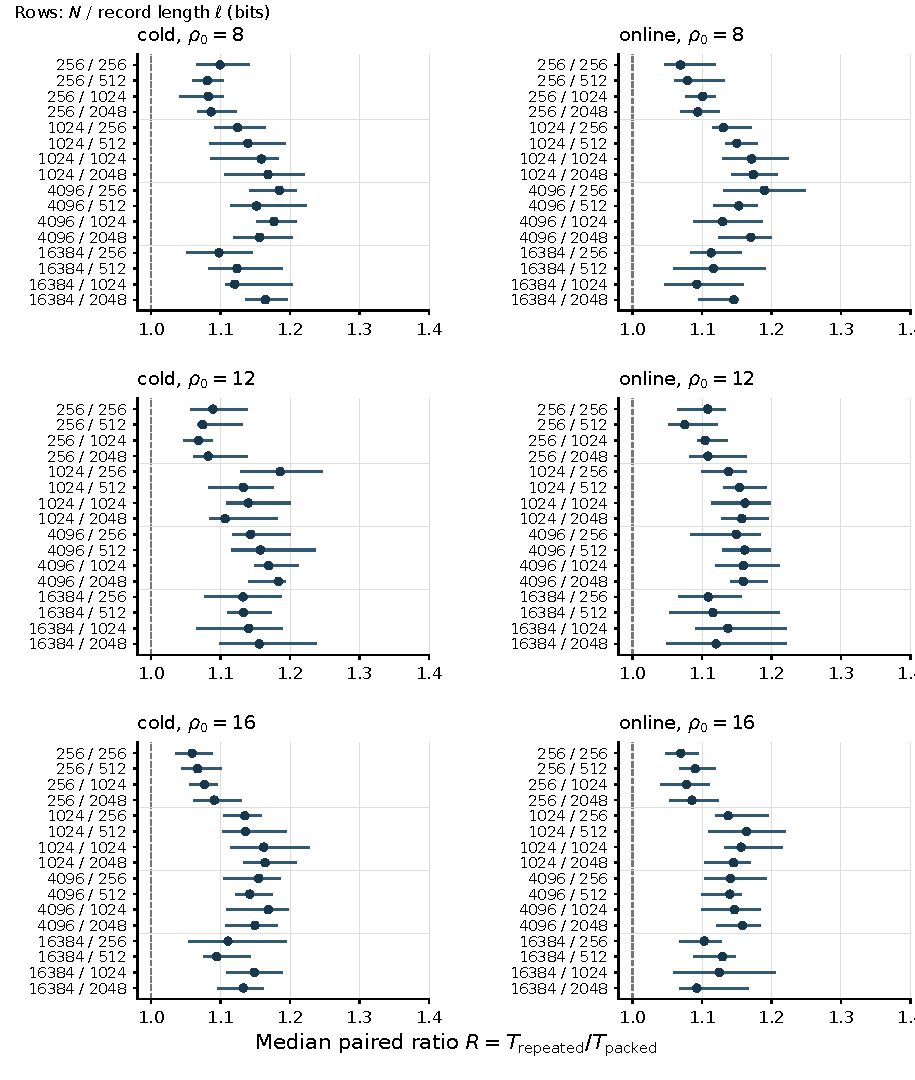
\includegraphics[width=\linewidth]{generated/primary.pdf}
\caption{Primary two-record comparison: all 96 cells. Points are median
paired repeated-to-packed task latency ratios; bars are pointwise 95\%
paired-bootstrap intervals. Cells remain separate; the figure makes no
family-wise or across-grid inference.}
\label{fig:primary-performance}
\end{figure}

\begin{table}[tbp]
\centering\small
\caption{Absolute task latency at the smallest and largest primary workload corners, with $\rho_0=8$. These four cells are descriptive examples; Fig.~\ref{fig:primary-performance} retains the full grid.}
\label{tab:absolute}
\setlength{\tabcolsep}{4pt}
\begin{tabular}{@{}rrlrrr@{}}
\toprule
$N$ & $\ell$ (bits) & View & Packed (s) & Repeated (s) & Paired $R$ \\
\midrule
256 & 256 & cold & 0.206 & 0.223 & 1.099 \\
256 & 256 & online & 0.169 & 0.180 & 1.069 \\
16384 & 2048 & cold & 14.315 & 16.743 & 1.164 \\
16384 & 2048 & online & 12.036 & 13.509 & 1.146 \\
\bottomrule\end{tabular}
\par\smallskip\begin{minipage}{\linewidth}\footnotesize Time columns are separate method medians. Their quotient is not the median paired ratio in the last column.\end{minipage}
\end{table}


\subsection{Multiplicity Experiment}
\label{sec:multiplicity}
The multiplicity experiment varies \(\alpha\in\{2,3,4\}\) at
\(N\in\{1024,4096\}\), \(\ell\in\{512,2048\}\), \(\rho_0=8\) and
\(w=8\alpha\), again with \(L=1\). Packed execution is a serial worker
pinned to one logical CPU. Repeated execution uses \(\alpha\) private
workers on distinct logical CPUs from a four-CPU set, which also bounds
the parent. Each worker has an 8 GiB address-space limit; aggregate
virtual memory has a separately sampled 16 GiB limit. Both width and
repeated-worker CPU count change with multiplicity. This is not a
fixed-total-core scaling comparison, and visible WSL core IDs do not
establish physical host isolation.

All 24 observed median ratios exceed one. Pointwise intervals exclude
one in all eight cells at each of \(\alpha=3,4\), but only three of eight
at \(\alpha=2\). All eight fixed-workload/view rows have
\(R_2<R_3<R_4\) (Table~\ref{tab:multiplicity}); this ordering is descriptive,
without a monotonicity significance test or universal scaling claim.

The two-record entries are internal references for this experiment.
All eight are smaller than their matched primary-experiment ratios, with
disjoint experiment-specific intervals. Extraction scope, API wrappers,
affinity, parent allowance, fixtures and sample schedules differ. In
particular, the primary adapter reads record-used fields, while the
multiplicity adapter extracts complete polynomial blocks with checked
wrappers. These differences have no established causal attribution. The
experiments remain separate; neither estimate is selected as the true
effect, and their samples are not pooled.
\begin{table}[tbp]
\centering\small
\caption{Multiplicity experiment at $\rho_0=8$, $w=8\alpha$ and $L=1$. Each cell contains ten measured pairs. Entries are median paired ratios with pointwise 95\% intervals.}
\label{tab:multiplicity}
\setlength{\tabcolsep}{4pt}
\begin{tabular}{@{}rrlccc@{}}
\toprule
$N$ & $\ell$ (bits) & View & $\alpha=2$ & $\alpha=3$ & $\alpha=4$ \\
\midrule
1024 & 512 & cold & \shortstack{1.050\\\scriptsize [1.005, 1.078]} & \shortstack{1.098\\\scriptsize [1.038, 1.129]} & \shortstack{1.140\\\scriptsize [1.119, 1.184]} \\[3pt]
1024 & 512 & online & \shortstack{1.055\\\scriptsize [1.030, 1.082]} & \shortstack{1.092\\\scriptsize [1.077, 1.107]} & \shortstack{1.151\\\scriptsize [1.106, 1.235]} \\[3pt]
1024 & 2048 & cold & \shortstack{1.036\\\scriptsize [1.006, 1.056]} & \shortstack{1.114\\\scriptsize [1.078, 1.137]} & \shortstack{1.154\\\scriptsize [1.117, 1.186]} \\[3pt]
1024 & 2048 & online & \shortstack{1.033\\\scriptsize [0.980, 1.067]} & \shortstack{1.096\\\scriptsize [1.074, 1.130]} & \shortstack{1.121\\\scriptsize [1.088, 1.143]} \\[3pt]
4096 & 512 & cold & \shortstack{1.025\\\scriptsize [1.000, 1.052]} & \shortstack{1.093\\\scriptsize [1.039, 1.106]} & \shortstack{1.122\\\scriptsize [1.095, 1.144]} \\[3pt]
4096 & 512 & online & \shortstack{1.024\\\scriptsize [0.998, 1.039]} & \shortstack{1.065\\\scriptsize [1.043, 1.083]} & \shortstack{1.108\\\scriptsize [1.094, 1.138]} \\[3pt]
4096 & 2048 & cold & \shortstack{1.013\\\scriptsize [0.986, 1.026]} & \shortstack{1.071\\\scriptsize [1.061, 1.080]} & \shortstack{1.129\\\scriptsize [1.110, 1.152]} \\[3pt]
4096 & 2048 & online & \shortstack{1.015\\\scriptsize [0.993, 1.034]} & \shortstack{1.066\\\scriptsize [1.053, 1.078]} & \shortstack{1.117\\\scriptsize [1.097, 1.158]} \\[3pt]
\bottomrule\end{tabular}
\par\smallskip\begin{minipage}{\linewidth}\footnotesize The two-record entries are internal references for this experiment. Packed execution is serial; repeated tasks use $\alpha$ concurrent workers. This is not a fixed-total-core comparison.\end{minipage}
\end{table}


\subsection{Bundle Sensitivity and Capacity}
\label{sec:capacity-evaluation}
The sensitivity experiment crosses two extraction/API bundles
(record-field and full-block) with the primary two-CPU and multiplicity
four-CPU-parent resource allowances. It holds \(N=1024\), \(\ell=512\),
\(\alpha=2\), \(\rho_0=8\) and the fixture generation rule fixed. Rebuilt
source variants retain their wrapper and extraction differences; resource
bundles include affinity and memory limits. A common runner records
monitor timestamps at a nominal 10 ms cadence; monitoring overhead has
not been shown to be zero. Extra record-field
coefficient validation occurs outside task timing. These are bundle
comparisons, not isolated changes to one operation.

The sensitivity and capacity designs were fixed before formal timing.
Each cell has three successive sessions, with three warmup and ten
measured pairs per session, balanced five/five method order and
interleaved cells. Cells do not execute concurrently, and pilot observations
are excluded. A failed or missing warmup
withholds that cell/session's latency summary; stopping rules retain
failed, incomplete and unstarted tasks and forbid effect-dependent sample
changes. All 702 scheduled pairs completed, including 540 measured pairs.
The reported intervals for these experiments are observed ranges of
three session medians, not confidence intervals or independent-day
replication.

Sensitivity median ratios range from 1.123 to 1.236. In each view and
implementation bundle, the descriptive median is larger under the
two-CPU resource allowance. The implementation ordering changes with
resource bundle and view. The two implementations' session ranges overlap
within each fixed resource bundle and view. The supplemental
table preserves all eight cells. These observations do not uniquely
explain the primary/multiplicity difference.

\paragraph{Two distinct capacity boundaries.}
Let \(u=\alpha J/n\). For \(L=1\), a coefficient-position representation
of the same fixed segments is
\[
 PM_{\rm position}(X)=\sum_{\nu=1}^{\alpha}
 X^{(\nu-1)J}P_{i_\nu}(X).
\]
It fits without overlapping coefficient ranges when \(\alpha J\le n\).
Radix packing uses coefficient values instead, subject to
\(t\ge B^\alpha\), no-wrap and native constraints. The quantity
\(\lceil\alpha J/n\rceil\) is a coefficient-slot lower bound, not the
reply count or runtime of an implemented alternative protocol. Other
encodings and hybrid schemes are not ruled out.

The boundary \(u=1\) differs from \(J=n\), where an individual record
starts to require more blocks. The capacity experiment fixes
\(N=1024\), \(\alpha=4\), \(\rho_0=8\), \(w=32\), full-block extraction
and the four-CPU parent allowance. Four lengths cross \(u=1\) while
retaining \(L=1\); a fifth has \(L=2\) (Table~\ref{tab:capacity}). All ten
median ratios exceed one, ranging from 1.258 to 1.339, without monotone
ordering in record length. These results establish finite capacity
coverage, not the speed of a coefficient-position comparator.
\begin{table}[tbp]
\centering\small
\caption{Capacity experiment: $N=1024$, $\alpha=4$, $\rho_0=8$, $w=32$, full-block extraction and the four-CPU parent allowance. Entries are median paired ratios with observed ranges of three session medians.}
\label{tab:capacity}
\setlength{\tabcolsep}{4pt}
\begin{tabular}{@{}rrrrcc@{}}
\toprule
$\ell$ (bits) & $J$ & $L$ & $u$ & Cold & Online \\
\midrule
4096 & 512 & 1 & 0.5 & 1.339 [1.312, 1.376] & 1.308 [1.232, 1.360] \\
8192 & 1024 & 1 & 1 & 1.311 [1.284, 1.318] & 1.271 [1.268, 1.286] \\
12288 & 1536 & 1 & 1.5 & 1.311 [1.277, 1.336] & 1.287 [1.287, 1.299] \\
16384 & 2048 & 1 & 2 & 1.319 [1.293, 1.337] & 1.258 [1.257, 1.266] \\
65536 & 8192 & 2 & 8 & 1.294 [1.275, 1.310] & 1.305 [1.293, 1.310] \\
\bottomrule\end{tabular}
\par\smallskip\begin{minipage}{\linewidth}\footnotesize Each cell has 30 measured pairs. Brackets are descriptive session ranges, not confidence intervals. Query buffers are 128/512 MiB for packed/repeated; reply buffers are 128/512 KiB for $L=1$ and 256/1024 KiB for $L=2$.\end{minipage}
\end{table}


\subsection{Payload and Resource Accounting}
For a declared ciphertext representation of size \(|C|\),
\begin{equation}\label{eq:payload}
 |Q|=N|C|,\qquad |\mathsf{Resp}|=L|C|.
\end{equation}
One native ciphertext occupies 131,072 bytes: two components, two RNS
limbs and 4096 64-bit words. Repeated retrieval copies \(\alpha N\)
query ciphertexts and \(\alpha L\) reply ciphertexts. These native
buffers are exactly \(\alpha\) times their packed counterparts, but
transport, framing, metadata and key distribution are unmeasured.
Canonical mathematical serialization can have a different size.

For byte-aligned records the raw database is \(N\ell/8\) bytes, counted
once regardless of multiplicity. The packed query remains larger than
this database at every reported length (Table~\ref{tab:payload}); even
at \(\ell=65536\) its ratio to raw size is 16. Thus same-profile buffer
savings do not establish raw-download or wire-traffic superiority.
\begin{table}[tbp]
\centering\small
\caption{Exact native buffer accounting for representative byte-aligned workloads with $\rho_0=8$. P/R denotes packed/repeated retrieval. Raw database size counts each record once.}
\label{tab:payload}
\setlength{\tabcolsep}{4pt}
\begin{tabular}{@{}rrrrcc@{}}
\toprule
$N$ & $\ell$ (bits) & $\alpha$ & Raw (KiB) & Query P/R (MiB) & Reply P/R (KiB) \\
\midrule
256 & 256 & 2 & 8 & 32/64 & 128/256 \\
16384 & 2048 & 2 & 4096 & 2048/4096 & 128/256 \\
1024 & 8192 & 4 & 1024 & 128/512 & 128/512 \\
1024 & 16384 & 4 & 2048 & 128/512 & 128/512 \\
1024 & 65536 & 4 & 8192 & 128/512 & 256/1024 \\
\bottomrule\end{tabular}
\par\smallskip\begin{minipage}{\linewidth}\footnotesize One ciphertext occupies 128 KiB. These are in-memory buffer sizes; transport, framing and metadata are unmeasured.\end{minipage}
\end{table}


Aggregate CPU work sums worker user-plus-system time, excluding parent
CPU. In the multiplicity experiment, repeated-to-packed ratios of
separate CPU medians are 1.972--2.052, 3.033--3.149 and 4.085--4.295 for
\(\alpha=2,3,4\). They describe work, not latency or a fitted scaling law.
Repeated RSS sums worker lifetime peaks, an upper bound rather than a
synchronized peak; online staging remains included and parent RSS is
separate. Phase sums likewise do not identify critical-path contributions.
Full summaries and machine-readable mappings accompany the supplement.

\section{Discussion and Limitations}
\label{sec:discussion}
\paragraph{Formal and native scope.}
The formal result separates conditional recovery from single-challenge
index privacy. The latter assumes distribution-specific uniform-secret
PLWE hardness and efficient sampling; it neither follows from empirical
correctness nor requires a successful decryption event. The rounded
Gaussian width remains symbolic. Its exact efficient machine realization,
approximation and computational randomness require independent evidence.
The native bounded, biased sampler and OS-seeded PRNG have not been
bridged to that law, and a public native noise parameter is not a proved
absolute bound on integer coefficients. Consequently neither finite
native passes nor the parametric bound supplies a native negligible-failure
claim or a contemporary concrete-security certificate.

After a suitable joint-law and implementation bridge, task accounting
could take the form
\(\epsilon_{\rm task}\le\epsilon_{\rm dec}+d_{\rm joint}
+\epsilon_{\rm other}\), with separately justified sampling, abort and
runtime terms. An abort included in the joint-law distance is not counted
again. PRNG replacement needs a separate computational failure-test bound.
No such bound is established here. Independent repeated requests must
also share one complete-task reliability budget, as detailed in the
supplement. The privacy game gives neither symmetric PIR nor protection
against malicious replies, adaptive key reuse or decryption oracles.

\paragraph{Empirical generality.}
The measurements cover one flat backend path, one WSL2 host and finite
workloads. The comparator uses concurrent private workers under the same
profile within each experiment; it is not a globally optimized XPIR
service with shared persistent preprocessing. External PIR timings are
not aligned measurements. The capacity study adds one two-block length,
and bundle sensitivity covers only one workload. Neither supports
arbitrary-block, cross-host or bare-metal extrapolation.

The primary and multiplicity resource limits were enforced by their
runners, but individual monitoring samples were not retained. Their
transient virtual-memory and swap behavior cannot be reconstructed from
the surviving endpoints and summaries. The sensitivity/capacity data
retain actual monitor timestamps, yet sampled maxima are still not
instantaneous peaks. This difference limits resource diagnosis without
establishing invalidity of the recorded task times. Bootstrap intervals
are pointwise; three successive sessions give descriptive variation.
The unexplained two-record effect difference remains part of the evidence.

\paragraph{Design tradeoff.}
Radix packing places several bounded values in each coefficient without
bucket placement or additional SIMD rotations, while consuming plaintext
capacity and no-wrap margin. It retains a linear-size query and does not
claim general communication efficiency. A deployment would require a
joint choice of correctness and security parameters, a justified sampler
and randomness implementation, transport measurements, and comparisons
with optimized preprocessing and query-compression alternatives.

\section{Conclusion}
\label{sec:conclusion}
Radix-packed retrieval combines bounded segments from several records
within each reply coefficient while retaining an XPIR-style linear
interface. Its specification makes encoding, exact capacity, integer
no-wrap correctness and single-challenge privacy explicit. The privacy
reduction uses \(N+1\) uniform-secret PLWE samples and the stated
unit-probability loss; the full-task reliability bound remains parametric
in the specified rounded Gaussian law.

On the measured WSL2 host, the primary two-record comparison finds lower
median completed-task latency than concurrent same-profile repeated XPIR
throughout the tested grid. Separate multiplicity, sensitivity and
capacity experiments describe additional finite regimes, including one
two-block workload. Native buffer savings remain relative to repeated
execution; the flat query still exceeds raw database size at these lengths.
The unresolved native/formal bridge, distinct experimental resource
contracts and unmeasured transport delimit the conclusions.

\section*{Artifact availability}
The accompanying reproduction package contains the manuscript sources,
archived observations, frozen analysis, new presentation code and
build/functional validation instructions. Its release identity and
verification status are recorded in the package documentation.

\bibliographystyle{elsarticle-num}
\bibliography{references}
\appendix
\section{Supporting Proofs}
\label{app:proofs}
\subsection{Rounded-noise tails}
\label{app:lem-rounded-tail}
\begin{proof}
The rounding cells for \(-h,\ldots,h\) fill
\([-h-1/2,h+1/2)\), apart from boundary conventions. Hence
\(|Z|>h\) iff \(|Y|\ge h+1/2\), up to half-integer ties,
which have probability zero under the continuous Gaussian.
Integrating its two symmetric tails proves \eqref{eq:rounded-strict-tail}.
The non-strict identity follows from integer-valuedness:
\(|Z|\ge h\) iff \(|Z|>h-1\).
\end{proof}

\subsection{Block-support noise bound}
\label{app:lem-block-noise}
\begin{proof}
There are \(m_j\) valid segment positions in block \(j\), each in
\([0,B-1]\), and all other coefficients are zero. Since
\((L-1)n<J\le Ln\), actual blocks are nonempty. Unused high bits in the
last segment only reduce the stated bound.
For degree-\(<n\) representatives, the coefficient of a negacyclic product is
\[
 [X^k](Pe)=\sum_{u+v=k}P_u e_v-\sum_{u+v=k+n}P_u e_v.
\]
The minus sign is exactly the reduction \(X^n=-1\).
For each \(u\) there is one \(v=(k-u)\bmod n\) in these two sums.
The triangle inequality therefore bounds its absolute value by
\(\sum_u|P_u|\|e\|_\infty\).
On \(G_h\), each \(\|e_i\|_\infty\le h\); summing
\(\|\widehat P_{i,j}e_i\|_\infty\le m_j(B-1)h\) over all \(N\) records
proves \eqref{eq:aggregate-good-event-bound}.
\end{proof}

\subsection{Normal-form specialization}
\label{app:normal-form}
\begin{proof}[Specialization sketch]
Given \((a_i,b_i)_{i=0}^{\tau}\), output zero if \(a_0\) is not a unit.
Otherwise give \(\mathcal D\) the pairs
\[
 A_i=-a_0^{-1}a_i,\qquad B_i=b_i+A_i b_0,\quad i\in[\tau].
\]
In the real case, \(B_i=A_i e_0+e_i\), so the new shared secret is
\(e_0\leftarrow\chi\) and all remaining errors still have law \(\chi\).
The unit event depends only on \(a_0\), hence does not bias \(e_0\);
unit multiplication preserves the independent uniform \(A_i\).
In the uniform case, conditional on \(a_0,b_0\) and the unit event,
the transformed pairs are independent uniform pairs.
Thus \(\mathcal B\)'s gap is exactly \(p_{\rm unit}\) times
\(\mathcal D\)'s gap. Unit testing and inversion are polynomial-time
operations: use the multiplication matrix of \(a_0\) over \(\mathbb Z_q\),
test whether its determinant is coprime to \(q\), and invert when it is.
No factorization of \(q\) is required.
\end{proof}

\subsection{Ciphertext scaling and translation}
\label{app:ske}
\begin{proof}
For each normal-form pair \((A,B=As+E)\) and canonical message lift
\(\widehat m\), set
\[
 (a,b)=(tA,tB+\widehat m).
\]
Then \(b=as+tE+\widehat m\), exactly XPIR's SKE syntax, or
\(C=(b,-a)\) in our ordering. In the uniform branch,
\((tA,tU+\widehat m)\) remains uniform because \(t\) is a unit modulo \(q\).
Apply the same bijection to all samples sharing \(s\).
This is the noise-scaling observation of
\cite[Proposition~1]{homomorphic}, followed by message translation;
the argument uses only \(\gcd(t,q)=1\), including for composite \(q\).
\end{proof}

\subsection{Single-challenge privacy reduction}
\label{app:privacy}
\begin{proof}
First construct a normal-form distinguisher \(\mathcal D\).
Given \(pp\) and \(N\) normal-form-or-uniform pairs \((A_i,B_i)\),
it runs \(\mathcal A_1(pp)\) to obtain \((M,I_0,I_1,\sigma)\). If the inputs are
illegal, it outputs a fair bit, matching the experiment's convention.
Otherwise it privately chooses \(\beta\leftarrow\{0,1\}\) and forms
\begin{equation}
\label{eq:reduction-query}
 C_i=(tB_i+v_{I_\beta,i},-tA_i),\qquad Q=(C_1,\ldots,C_N).
\end{equation}
The constants \(v_{I_\beta,i}\) use their canonical message lifts.
It computes \(P=\mathsf{DBEncode}(M)\) and
\(\mathsf{Resp}=\mathsf{ReplyGen}(pp,P,Q)\), gives
\((Q,\mathsf{Resp})\) to \(\mathcal A_2\) with precisely the other inputs
of the experiment, and outputs one iff the guess \(\beta'\) equals \(\beta\).
It needs neither \(s\) nor an encryption or decryption oracle.

For real normal-form samples, \(B_i=A_i s+E_i\), with one shared
\(s\leftarrow\chi\) and fresh independent \(E_i\leftarrow\chi\).
By Corollary~\ref{cor:ske-pseudorandom}, setting \(a_i=tA_i\) gives
\[
 C_i=(a_i s+tE_i+v_{I_\beta,i},-a_i),
\]
exactly a fresh \(\mathsf{Enc}_s(v_{I_\beta,i})\). This preserves the
entire joint law of all \(N\) query ciphertexts, including their shared
secret, not just individual marginals. The first-stage output has the
same law as in the game because it depends only on \(pp\) and adversary
randomness, independently of the samples and of \(\beta\).
The encoded database and reply use the actual deterministic protocol
algorithms. Hence \((Q,\mathsf{Resp})\) has exactly the formal protocol
view's distribution, and
\[
 \Pr[\mathcal D(pp,\mathcal F_{\rm real}^{(N)})=1]
   =\Pr[\text{privacy experiment succeeds}].
\]

For uniform samples, \(A_i,B_i\) are independent uniform ring elements.
Multiplication by the unit \(t\), negation, and translation by the fixed
\(v_{I_\beta,i}\) preserve uniformity. Conditional on every legal first-stage
output and either value of \(\beta\), the entire query is uniform in
\((R_q^2)^N\), independently of \(\beta\). The reply is deterministic PPT
post-processing of this query and the fixed database. Therefore
\((Q,\mathsf{Resp})\) remains independent of \(\beta\).
The same is true of the adversary's resulting guess. Accounting also
for the independent fair output on illegal input,
\[
 \Pr[\mathcal D(pp,\mathcal F_{\rm unif}^{(N)})=1]=\tfrac12.
\]
Under the success-minus-\(1/2\) convention of the privacy game and the
acceptance-gap convention for PLWE, subtraction yields
\[
 \Adv^{\rm priv}_{\Pi,\mathcal A}(\kappa)
 =\Adv^{\rm NF}_{\mathcal D}(\kappa;N).
\]
Compose \(\mathcal D\) with Corollary~\ref{cor:normal-form} at \(\tau=N\)
to obtain \(\mathcal B\). It consumes \(N+1\) uniform-secret ring samples,
uses the first for normal form, and passes the remaining \(N\) transformed
pairs to \(\mathcal D\). Conditional on the unit event its simulation is
the one just analyzed. With output zero on abort, its uniform-branch
acceptance probability is \(p_{\rm unit}/2\), not \(1/2\); both branches
are scaled by the same \(p_{\rm unit}\). Thus
\[
 \Adv^{\rm uPLWE}_{\mathcal B}(\kappa;N+1)
 =p_{\rm unit}\,\Adv^{\rm NF}_{\mathcal D}(\kappa;N),
\]
which gives the stated bound. There is no extra factor \(2\), \(N\), or
\(2\alpha\): the reduction simulates the joint query in one step.

All steps are polynomial-time: the normal-form operations are as in
Corollary~\ref{cor:normal-form}, both adversary stages are PPT, and
encoding and reply generation operate on a polynomial-size database
and query using polynomially many ring operations with polynomial
bit complexity. Deterministic reply generation adds no distinguishing loss.
\end{proof}

\end{document}
